% ============================================================================
% Lecture 06 (B05): Deep Equilibrium Nets --- The Central Idea
% Deep Learning for Solving and Estimating Dynamic Models in Economics and Finance
% Course author: Simon Scheidegger
% ============================================================================

\documentclass[aspectratio=169,11pt]{beamer}

% ---------- Theme and colors ----------
\usecolortheme{dove}
\setbeamertemplate{navigation symbols}{}
\setbeamertemplate{footline}{%
  \hfill\usebeamerfont{page number in head/foot}%
  \usebeamercolor[fg]{normal text}%
  \insertframenumber\,/\,\inserttotalframenumber\kern1em\vskip4pt}
\setbeamerfont{frametitle}{size=\huge}

% ---------- Packages ----------
\usepackage[utf8]{inputenc}
\usepackage[T1]{fontenc}
\usepackage{amsmath,amssymb,amsfonts}
\usepackage{bm}
\usepackage{graphicx}
\usepackage{tikz}
\usetikzlibrary{shapes,arrows.meta,positioning,calc,fit,backgrounds,patterns,decorations.pathreplacing}
\usepackage{pgfplots}
\pgfplotsset{compat=1.18}
\usepackage{booktabs}
\usepackage{hyperref}
\usepackage{multicol}
\usepackage{xcolor}
\usepackage{algorithm}
\usepackage{algorithmic}

% ---------- Custom colors ----------
\definecolor{uzhblue}{rgb}{0,0,0.5}
\definecolor{uzhgreylight}{RGB}{236,238,241}
\definecolor{uzhgreydark}{RGB}{81,86,94}
\definecolor{harvardcrimson}{RGB}{153,0,0}
\definecolor{unil@blue}{RGB}{0,140,204}
\definecolor{unil@black}{RGB}{35,31,32}
\definecolor{darkgreen}{RGB}{0,100,0}
\definecolor{darkred}{RGB}{139,0,0}
\definecolor{softblue}{RGB}{70,130,180}
\definecolor{softorange}{RGB}{230,159,0}
\definecolor{softgreen}{RGB}{0,158,115}

% ---------- Set beamer colors ----------
\setbeamercolor{frametitle}{bg=uzhgreylight, fg=uzhblue}
\setbeamercolor{title}{fg=uzhblue}
\setbeamercolor{structure}{fg=uzhblue}
\setbeamercolor{block title}{bg=unil@blue, fg=white}
\setbeamercolor{block body}{bg=uzhgreylight}
\setbeamercolor{block title alerted}{bg=darkred,fg=white}
\setbeamercolor{block body alerted}{bg=red!5}
\setbeamercolor{block title example}{bg=darkgreen,fg=white}
\setbeamercolor{block body example}{bg=green!5}
\setbeamercolor{item}{fg=unil@black}
\setbeamercolor{normal text}{fg=unil@black}

% ---------- Emphasis and hyperlinks ----------
\newcommand{\emphc}[1]{\textcolor{harvardcrimson}{#1}}
\hypersetup{colorlinks,linkcolor=harvardcrimson,urlcolor=harvardcrimson}

% ---------- Math commands ----------
\newcommand{\x}{\bm{x}}
\newcommand{\w}{\bm{w}}
\newcommand{\bb}{\bm{b}}
\newcommand{\z}{\bm{z}}
\newcommand{\W}{\bm{W}}
\newcommand{\X}{\bm{X}}
\renewcommand{\a}{\bm{a}}
\newcommand{\R}{\mathbb{R}}
\newcommand{\E}[1]{\mathbb{E}\!\left[#1\right]}
\DeclareMathOperator*{\argmin}{arg\,min}
\DeclareMathOperator*{\argmax}{arg\,max}

% ---------- Title ----------
\title[Lecture 08 (B07)]{Lecture 08 (B07): Brock--Mirman --- Uncertainty and Numerical Integration}
\subtitle{Residuals, expectations, Gauss--Hermite and monomial quadrature, training diagnostics}
\author{Simon Scheidegger}
\institute{HEC, University of Lausanne}
\date{}
\begin{document}

% Custom command used in some "Finger Exercise" frame titles.
\providecommand{\exercisepause}{%
  \tikz[baseline=(X.base)]{\node[fill=darkgreen!80!black, text=white,
  rounded corners=2pt, inner sep=3pt, font=\scriptsize\bfseries](X){PAUSE};}}

{\setbeamercolor{background canvas}{bg=uzhgreylight}
\begin{frame}
\titlepage
\end{frame}
}

\begin{frame}{Brock--Mirman: Residual, Expectation, Loss}
\textbf{Pathwise residual used in the notebook} (full-depreciation $\delta=1$ benchmark):
\[
G_t = 1 - \beta \, \frac{C_t}{C_{t+1}} \cdot \alpha z_{t+1} K_{t+1}^{\alpha-1},
\]
with
\[
K_{t+1} = s_t z_t K_t^\alpha, \qquad
C_{t+1} = (1-s_{t+1}) z_{t+1} K_{t+1}^\alpha.
\]

\vspace{-0.2em}
{\scriptsize\emphc{Partial depreciation.}  The uncertainty notebook uses $\delta=0.1$; the marginal productivity of capital then becomes $\alpha z_{t+1} K_{t+1}^{\alpha-1} + (1-\delta)$ and $K_{t+2} = z_{t+1} K_{t+1}^{\alpha} + (1-\delta) K_{t+1} - C_{t+1}$.  The closed-form $\phi = \alpha\beta$ only holds at $\delta=1$.}

\vspace{0.3em}
\begin{columns}[T]
\column{0.52\textwidth}
\textbf{Training loss:}
\[
\ell_\rho = \frac{1}{N}\sum_{i=1}^{N} |G_t^{(i)}|^2.
\]

\begin{itemize}
    \setlength{\itemsep}{1pt}
    \item Simulate states $(K_t,z_t)$ forward
    \item Draw one next-period shock $z_{t+1}$ per state
    \item Average $G_t^2$ over many simulated states
\end{itemize}

\column{0.44\textwidth}
\begin{block}{Expectation Handling}
\small
\textbf{Brock--Mirman notebook:} path averaging, one shock per state.\\[2pt]
\textbf{Richer models:} approximate the conditional expectation explicitly via \emphc{quadrature}, see next three slides.
\end{block}
\end{columns}
\end{frame}

% ============================================================================
% INTERLUDE: QUADRATURE RULES FOR CONDITIONAL EXPECTATIONS
% ============================================================================

% --- Slide 29: Numerical integration primer (motivation + two pictures) ---
\begin{frame}{Numerical Integration: Why and How}
\scriptsize
\textbf{Why an integral always shows up.} Euler equations, Bellman operators, REE diagnostics, climate damages, structural moments, all reduce to evaluating
\(
\mathbb{E}[g(\bm\varepsilon)] = \int g(\bm\varepsilon)\,\mu(\bm\varepsilon)\,d\bm\varepsilon.
\)
Closed forms are rare, so we approximate by $\sum_q w_q\, g(\bm\varepsilon_q)$. Two paradigms underlie every rule.

\vspace{0.2em}
\begin{columns}[T]
\column{0.54\textwidth}
\begin{center}
{\scriptsize\textbf{Deterministic: tile the area, integral $\to$ sum}}\\[1pt]
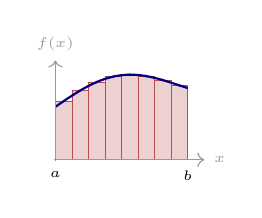
\begin{tikzpicture}[scale=0.42, font=\tiny]
    \foreach \i in {0,1,2,3,4,5,6,7} {
        \pgfmathsetmacro{\mx}{0.5*\i + 0.25}
        \pgfmathsetmacro{\hh}{1.6 + 0.6*sin(deg(\mx*0.85)) + 0.18*\mx}
        \draw[fill=harvardcrimson!18, draw=harvardcrimson!70, very thin]
            (0.5*\i, 0) rectangle (0.5*\i + 0.5, \hh);
        \fill[harvardcrimson] (\mx, \hh) circle (1.2pt);
    }
    \draw[thick, uzhblue, smooth, samples=80, domain=0:4]
        plot(\x, {1.6 + 0.6*sin(deg(\x*0.85)) + 0.18*\x});
    \draw[->, gray!80] (-0.05,0) -- (4.5,0) node[right, font=\tiny] {$x$};
    \draw[->, gray!80] (0,-0.05) -- (0,3.0) node[above, font=\tiny] {$f(x)$};
    \node[below, font=\tiny] at (0,-0.05) {$a$};
    \node[below, font=\tiny] at (4,-0.05) {$b$};
\end{tikzpicture}
\end{center}
\vspace{-0.6em}
{\tiny
With $\Delta x = (b-a)/N$, $x_i = a + i\Delta x$, $I = \int_a^b\! f(x)\,dx \approx \sum_i w_i\, f(x_i)$:
\vspace{-0.3em}
\begin{itemize}\itemsep0pt\setlength{\leftmargini}{1em}
    \item \emphc{Midpoint:} $I_N^{\text{mid}} = \Delta x \sum_{i=1}^N f(x_i^{\text{mid}})$, $\mathcal{O}(N^{-2})$
    \item \emphc{Trapezoid:} $I_N^{\text{trap}} = \tfrac{\Delta x}{2}\bigl[f(x_0) + 2\!\sum_{i=1}^{N-1}\!f(x_i) + f(x_N)\bigr]$, $\mathcal{O}(N^{-2})$
    \item \emphc{Simpson:} parabolic arcs through triples, $\mathcal{O}(N^{-4})$
    \item \emphc{Gauss--Hermite:} optimal nodes/weights for $e^{-x^2}$, $\mathcal{O}(N^{-(2Q-1)})$
\end{itemize}
}
{\tiny $d$-dim Cartesian grid: cost $\mathcal{O}(N^d)$, \emphc{curse of dimensionality}.}

\column{0.42\textwidth}
\begin{center}
{\scriptsize\textbf{Random: throw darts to estimate $\pi$}}\\[1pt]
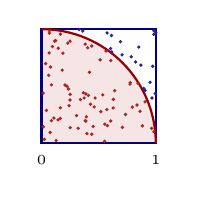
\begin{tikzpicture}[scale=1.45, font=\tiny]
    \fill[harvardcrimson!10] (0,0) -- (1,0) arc(0:90:1) -- cycle;
    \draw[thick, uzhblue] (0,0) rectangle (1,1);
    \draw[thick, harvardcrimson] (1,0) arc (0:90:1);
    \pgfmathsetseed{42}
    \foreach \i in {1,...,100} {
        \pgfmathsetmacro{\xx}{rnd}
        \pgfmathsetmacro{\yy}{rnd}
        \pgfmathsetmacro{\rsq}{\xx*\xx + \yy*\yy}
        \pgfmathparse{\rsq < 1 ? 1 : 0}
        \edef\inside{\pgfmathresult}
        \ifnum\inside=1
          \fill[harvardcrimson!85] (\xx,\yy) circle (0.016);
        \else
          \fill[uzhblue!85] (\xx,\yy) circle (0.016);
        \fi
    }
    \node[below, font=\tiny] at (0,-0.02) {$0$};
    \node[below, font=\tiny] at (1,-0.02) {$1$};
\end{tikzpicture}
\end{center}
\vspace{-0.4em}
{\tiny
Throw $N$ uniform darts at $\Omega = [0,1]^2$:
\[
\frac{\pi}{4} \;=\; \!\!\int_0^1\!\!\!\int_0^1\!\! \mathbf{1}[x^2+y^2 \le 1]\,dx\,dy \;\approx\; \frac{N_{\mathrm{in}}}{N}
\]
\vspace{-1.2em}
\[
\widehat{\pi}_N = 4 N_{\mathrm{in}}/N, \quad \text{error } \mathcal{O}(N^{-1/2})
\]
\emphc{Independent of dimension}, but slow.
}
\end{columns}
\end{frame}

% --- Slide 30: Gauss-Hermite quadrature ---
\begin{frame}{Quadrature, I: Gauss--Hermite}
\footnotesize
\textbf{Setup.} Generic shock dimension $d$, with $\bm\varepsilon' \sim \mathcal{N}(0, I_d)$.  Brock--Mirman has $d=1$ (one productivity shock); the IRBC chapter will use $d=N+1$ ($N$ country shocks plus one aggregate).  We develop the framework here so it is ready for both cases.

\vspace{0.3em}
\textbf{One dimension.} Gauss--Hermite uses $Q$ nodes $\{\varepsilon_q\}$ (Hermite-polynomial roots) and weights $\{w_q\}$:
\[
\E{h(\varepsilon)} \;=\; \int_{-\infty}^{\infty} h(\varepsilon)\,\frac{e^{-\varepsilon^2/2}}{\sqrt{2\pi}}\,d\varepsilon \;\approx\; \sum_{q=1}^{Q} w_q\, h(\varepsilon_q),
\]
\emph{exact} for univariate polynomials of degree $\le 2Q-1$.

\vspace{0.3em}
\textbf{Tensor product in $d$ dimensions.} Combine 1D rules along each axis:
\[
\E{h(\bm\varepsilon')} \;\approx\; \sum_{q_1=1}^{Q}\!\!\cdots\!\!\sum_{q_d=1}^{Q} \Bigl(\textstyle\prod_{j} w_{q_j}\Bigr)\, h(\varepsilon_{q_1}, \ldots, \varepsilon_{q_d}).
\]
\vspace{-0.4em}
\begin{itemize}\itemsep1pt
    \item \emphc{Strength:} polynomial-exact in each coordinate, very accurate at low $d$.  For $d=1$ (Brock--Mirman) a $Q=3$ rule is essentially exact.
    \item \emphc{Weakness:} cost $Q^{d}$ blows up exponentially. For $Q=3$, $d=11$ (IRBC, $N=10$): $\sim 1.8\times 10^5$ nodes per state.
\end{itemize}
\end{frame}

% --- Slide 30: Monomial / Stroud-3 ---
\begin{frame}{Quadrature, II: Monomial (Stroud-3) Rule}
\footnotesize
\textbf{Idea.} Drop full polynomial-exactness in every coordinate, keep exactness for total degree $\le 3$. Place nodes only on the principal axes of the $d$-dimensional shock space:
\[
\boxed{\;
\E{h(\bm\varepsilon')} \;\approx\; \frac{1}{2d} \sum_{k=1}^{d} \Bigl[\, h\bigl(+\sqrt{d}\,\bm{e}_k\bigr) + h\bigl(-\sqrt{d}\,\bm{e}_k\bigr)\Bigr]
\;}
\]
where $\bm{e}_k$ is the $k$-th standard basis vector, giving $2d$ nodes at common radius $\sqrt{d}$.  For Brock--Mirman ($d=1$) this reduces to two nodes at $\pm 1$; for IRBC ($d=N+1$) it gives $2(N+1)$ nodes.

\vspace{0.5em}
\begin{columns}[T]
\column{0.52\textwidth}
\textbf{What it integrates exactly}
\begin{itemize}\itemsep1pt
    \item $\mathbb{E}[\varepsilon_i'] = \mathbb{E}[\varepsilon_i'^{\,3}] = 0$ ($\pm$-symmetry).
    \item $\mathbb{E}[\varepsilon_i' \varepsilon_j'] = 0$, $i \neq j$ (each node lies on one axis).
    \item $\mathbb{E}[\varepsilon_i'^{\,2}] = 1$ (variance preserved).
\end{itemize}
\textbf{Where it stops}
\begin{itemize}\itemsep1pt
    \item $\mathbb{E}[\varepsilon_i'^{\,4}]$ gives $d$ vs.\ truth $3$, a controlled fourth-order bias.
\end{itemize}

\column{0.46\textwidth}
\begin{block}{Why DEQNs love it}
\scriptsize
The integrand $h(\bm\varepsilon')$ is the policy network composed with model primitives, smooth and only mildly nonlinear. Degree-3 exactness is enough for Euler-error tolerances of $\sim\!10^{-3}$ on IRBC-class problems.\\[2pt]
\emphc{(Pichler 2011; Maliar \& Maliar 2014)}
\end{block}
\end{columns}
\end{frame}

% --- Slide 31: Cost comparison ---
\begin{frame}{Quadrature, III: Cost and Rules of Thumb}
\footnotesize
\textbf{Per-state quadrature cost} ($Q=3$ for the tensor-product rule):
\vspace{0.2em}
\begin{center}
\renewcommand{\arraystretch}{1.05}
\begin{tabular}{@{}rrrrl@{}}
\toprule
$N$ & shocks $N{+}1$ & tensor product $3^{N+1}$ & monomial $2(N{+}1)$ & speed-up\\
\midrule
$2$  & $3$  & $27$           & $6$   & $\sim\! 5\times$\\
$5$  & $6$  & $729$          & $12$  & $\sim\! 60\times$\\
$10$ & $11$ & $177{,}147$    & $22$  & $\sim\! 8{,}000\times$\\
$20$ & $21$ & $\sim\! 10^{10}$ & $42$  & $\sim\! 2\!\times\!10^8\times$\\
\bottomrule
\end{tabular}
\end{center}

\vspace{0.4em}
\begin{columns}[T]
\column{0.49\textwidth}
\begin{block}{Default rules of thumb}
\scriptsize
\begin{itemize}\itemsep1pt
    \item $N{+}1 \le 4$: tensor-product GH, $Q\!=\!5$.
    \item $5 \le N{+}1 \lesssim 30$: Stroud-3 monomial.
    \item $N{+}1 \gtrsim 30$ or fat-tailed integrands: QMC (Sobol $+$ inverse-CDF).
\end{itemize}
\end{block}

\column{0.49\textwidth}
\begin{block}{Practical notes}
\scriptsize
\begin{itemize}\itemsep1pt
    \item Only the quadrature \emphc{kernel} changes; same DEQN loss, same training loop.
    \item Validate by tightening the rule and checking the Euler-error histogram is stable.
    \item Full derivations: lecture script $\S 3.5$.
\end{itemize}
\end{block}
\end{columns}
\end{frame}

% --- Slide 32: Diagnostics ---
\begin{frame}{Diagnostics: How Do We Know Training Worked?}
\footnotesize
\textbf{Never trust a loss curve alone.}  On an independent \emph{test} simulation of the trained policy, run these four complementary checks:

\vspace{0.3em}
\begin{enumerate}\itemsep2pt
    \item \emphc{Euler-error distribution.}  Histogram $\log_{10}|e_{\mathrm{REE}}|$ on train and test states; both should peak near $10^{-3}$ or below, with no fatter right tail on test.
    \item \emphc{Policy-function benchmark.}  Overlay the DEQN policy on the analytic $s^\star=\beta\alpha$ for Brock--Mirman; for richer models, on a trusted reference (time iteration, perturbation).
    \item \emphc{Ergodic-set coverage.}  Scatter test states in the $(K_t,\log z_t)$ plane; the cloud should trace the training ergodic set~---~not collapse to a point, not spread like a grid.
    \item \emphc{Sanity checks.}  Verify accounting identities (budget, market clearing, non-negativity); check that ergodic moments (mean $K$, $\mathrm{std}(z)$, autocorrelations) match analytic or pre-computed values.
\end{enumerate}

\vspace{0.3em}
\begin{center}
{\scriptsize \emphc{Green flags:} low Euler error, matches benchmark, ergodic coverage, identities hold.\ \ \emphc{Red flags:} NaNs, fat tails, clamped policy, violated identities.}
\end{center}

\vspace{0.1em}
{\scriptsize When no closed-form benchmark exists, draw inspiration from the \emphc{VVUQ literature}~---~Verification, Validation \& Uncertainty Quantification (Roache 1998; Oberkampf \& Roy 2010; ASME V\&V 10/20)~---~which formalises residual convergence, solution verification, and error-bound reporting for computational models.}
\end{frame}

\end{document}
